
\documentclass[tikz,border=8pt]{standalone}
\usepackage{amsmath,amssymb}
\usetikzlibrary{positioning,arrows.meta,calc}
 
\definecolor{blockfill}{HTML}{EEEDFE}
\definecolor{blockdraw}{HTML}{534AB7}
\definecolor{blocktext}{HTML}{3C3489}
\definecolor{filmfill}{HTML}{E1F5EE}
\definecolor{filmdraw}{HTML}{0F6E56}
\definecolor{filmtext}{HTML}{085041}
\definecolor{neutfill}{HTML}{F1EFE8}
\definecolor{neutdraw}{HTML}{5F5E5A}

\begin{document}

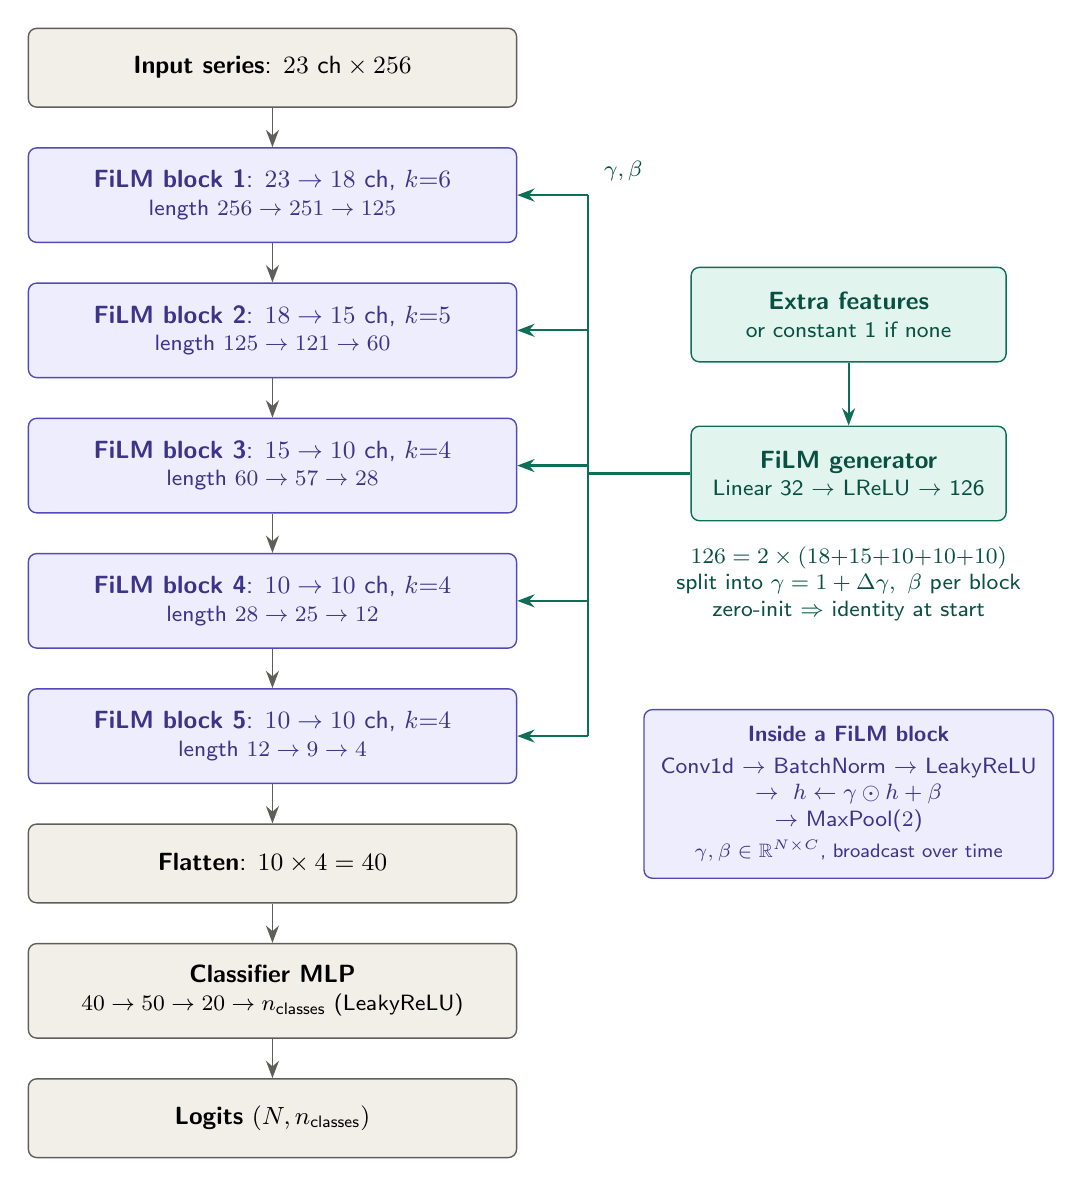
\begin{tikzpicture}[
    font=\sffamily\small,
    node distance=5mm,
    >={Stealth[length=2.2mm]},
    base/.style={rectangle, rounded corners=3pt, minimum width=62mm,
                 minimum height=10mm, align=center, line width=0.5pt},
    neutral/.style={base, fill=neutfill, draw=neutdraw},
    block/.style={base, fill=blockfill, draw=blockdraw, text=blocktext,
                  minimum height=12mm},
    film/.style={base, fill=filmfill, draw=filmdraw, text=filmtext,
                 minimum width=40mm, minimum height=12mm},
    flow/.style={->, draw=neutdraw, line width=0.6pt},
    mod/.style={->, draw=filmdraw, line width=0.8pt},
]
 
% ---------------- Main (series) path ----------------
\node[neutral] (in) {\textbf{Input series}: $23 \text{ ch} \times 256$};
 
\node[block, below=of in] (b1)
  {\textbf{FiLM block 1}: $23 \to 18$ ch, $k{=}6$\\[-1pt]
   {\footnotesize length $256 \to 251 \to 125$}};
\node[block, below=of b1] (b2)
  {\textbf{FiLM block 2}: $18 \to 15$ ch, $k{=}5$\\[-1pt]
   {\footnotesize length $125 \to 121 \to 60$}};
\node[block, below=of b2] (b3)
  {\textbf{FiLM block 3}: $15 \to 10$ ch, $k{=}4$\\[-1pt]
   {\footnotesize length $60 \to 57 \to 28$}};
\node[block, below=of b3] (b4)
  {\textbf{FiLM block 4}: $10 \to 10$ ch, $k{=}4$\\[-1pt]
   {\footnotesize length $28 \to 25 \to 12$}};
\node[block, below=of b4] (b5)
  {\textbf{FiLM block 5}: $10 \to 10$ ch, $k{=}4$\\[-1pt]
   {\footnotesize length $12 \to 9 \to 4$}};
 
\node[neutral, below=of b5] (flat) {\textbf{Flatten}: $10 \times 4 = 40$};
\node[neutral, below=of flat, minimum height=12mm] (cls)
  {\textbf{Classifier MLP}\\[-1pt]
   {\footnotesize $40 \to 50 \to 20 \to n_{\text{classes}}$ (LeakyReLU)}};
\node[neutral, below=of cls] (out) {\textbf{Logits} $(N, n_{\text{classes}})$};
 
\foreach \a/\b in {in/b1, b1/b2, b2/b3, b3/b4, b4/b5, b5/flat, flat/cls, cls/out}
  \draw[flow] (\a) -- (\b);
 
% ---------------- FiLM generator path ----------------
\coordinate (bus) at ($(b1.east)+(9mm,0)$);
 
\node[film, right=22mm of b2.east, anchor=west, yshift=2mm] (feat)
  {\textbf{Extra features}\\[-1pt]{\footnotesize or constant 1 if none}};
\node[film, below=8mm of feat] (gen)
  {\textbf{FiLM generator}\\[-1pt]{\footnotesize Linear 32 $\to$ LReLU $\to$ 126}};
\node[below=2mm of gen, align=center, text=filmtext, font=\sffamily\footnotesize] (note)
  {$126 = 2 \times (18{+}15{+}10{+}10{+}10)$\\
   split into $\gamma = 1 + \Delta\gamma,\ \beta$ per block\\
   zero-init $\Rightarrow$ identity at start};
 
\draw[mod] (feat) -- (gen);
 
% vertical bus from block 1 to block 5
\draw[filmdraw, line width=0.8pt] (bus |- b1.east) -- (bus |- b5.east);
\draw[filmdraw, line width=0.8pt] (gen.west) -- (bus |- gen.west);
 
\foreach \b in {b1, b2, b3, b4, b5}
  \draw[mod] (bus |- \b.east) -- (\b.east);
 
\node[text=filmtext, font=\sffamily\footnotesize, anchor=south west]
  at ($(bus |- b1.east)+(0.8mm,0.6mm)$) {$\gamma, \beta$};
 
% ---------------- Inset: inside one block ----------------
\node[below=10mm of note, align=center, draw=blockdraw, fill=blockfill,
      rounded corners=3pt, text=blocktext, inner sep=6pt, line width=0.5pt,
      font=\sffamily\footnotesize] (inset)
  {\textbf{Inside a FiLM block}\\[2pt]
   Conv1d $\to$ BatchNorm $\to$ LeakyReLU\\
   $\to\ h \leftarrow \gamma \odot h + \beta$\\
   $\to$ MaxPool($2$)\\[2pt]
   {\scriptsize $\gamma, \beta \in \mathbb{R}^{N \times C}$, broadcast over time}};
 
\end{tikzpicture}

\end{document}
